% Options for packages loaded elsewhere
% Options for packages loaded elsewhere
\PassOptionsToPackage{unicode}{hyperref}
\PassOptionsToPackage{hyphens}{url}
\PassOptionsToPackage{dvipsnames,svgnames,x11names}{xcolor}
%
\documentclass[
]{article}
\usepackage{xcolor}
\usepackage{amsmath,amssymb}
\setcounter{secnumdepth}{5}
\usepackage{iftex}
\ifPDFTeX
  \usepackage[T1]{fontenc}
  \usepackage[utf8]{inputenc}
  \usepackage{textcomp} % provide euro and other symbols
\else % if luatex or xetex
  \usepackage{unicode-math} % this also loads fontspec
  \defaultfontfeatures{Scale=MatchLowercase}
  \defaultfontfeatures[\rmfamily]{Ligatures=TeX,Scale=1}
\fi
\usepackage{lmodern}
\ifPDFTeX\else
  % xetex/luatex font selection
\fi
% Use upquote if available, for straight quotes in verbatim environments
\IfFileExists{upquote.sty}{\usepackage{upquote}}{}
\IfFileExists{microtype.sty}{% use microtype if available
  \usepackage[]{microtype}
  \UseMicrotypeSet[protrusion]{basicmath} % disable protrusion for tt fonts
}{}
\makeatletter
\@ifundefined{KOMAClassName}{% if non-KOMA class
  \IfFileExists{parskip.sty}{%
    \usepackage{parskip}
  }{% else
    \setlength{\parindent}{0pt}
    \setlength{\parskip}{6pt plus 2pt minus 1pt}}
}{% if KOMA class
  \KOMAoptions{parskip=half}}
\makeatother
% Make \paragraph and \subparagraph free-standing
\makeatletter
\ifx\paragraph\undefined\else
  \let\oldparagraph\paragraph
  \renewcommand{\paragraph}{
    \@ifstar
      \xxxParagraphStar
      \xxxParagraphNoStar
  }
  \newcommand{\xxxParagraphStar}[1]{\oldparagraph*{#1}\mbox{}}
  \newcommand{\xxxParagraphNoStar}[1]{\oldparagraph{#1}\mbox{}}
\fi
\ifx\subparagraph\undefined\else
  \let\oldsubparagraph\subparagraph
  \renewcommand{\subparagraph}{
    \@ifstar
      \xxxSubParagraphStar
      \xxxSubParagraphNoStar
  }
  \newcommand{\xxxSubParagraphStar}[1]{\oldsubparagraph*{#1}\mbox{}}
  \newcommand{\xxxSubParagraphNoStar}[1]{\oldsubparagraph{#1}\mbox{}}
\fi
\makeatother


\usepackage{longtable,booktabs,array}
\usepackage{calc} % for calculating minipage widths
% Correct order of tables after \paragraph or \subparagraph
\usepackage{etoolbox}
\makeatletter
\patchcmd\longtable{\par}{\if@noskipsec\mbox{}\fi\par}{}{}
\makeatother
% Allow footnotes in longtable head/foot
\IfFileExists{footnotehyper.sty}{\usepackage{footnotehyper}}{\usepackage{footnote}}
\makesavenoteenv{longtable}
\usepackage{graphicx}
\makeatletter
\newsavebox\pandoc@box
\newcommand*\pandocbounded[1]{% scales image to fit in text height/width
  \sbox\pandoc@box{#1}%
  \Gscale@div\@tempa{\textheight}{\dimexpr\ht\pandoc@box+\dp\pandoc@box\relax}%
  \Gscale@div\@tempb{\linewidth}{\wd\pandoc@box}%
  \ifdim\@tempb\p@<\@tempa\p@\let\@tempa\@tempb\fi% select the smaller of both
  \ifdim\@tempa\p@<\p@\scalebox{\@tempa}{\usebox\pandoc@box}%
  \else\usebox{\pandoc@box}%
  \fi%
}
% Set default figure placement to htbp
\def\fps@figure{htbp}
\makeatother


% definitions for citeproc citations
\NewDocumentCommand\citeproctext{}{}
\NewDocumentCommand\citeproc{mm}{%
  \begingroup\def\citeproctext{#2}\cite{#1}\endgroup}
\makeatletter
 % allow citations to break across lines
 \let\@cite@ofmt\@firstofone
 % avoid brackets around text for \cite:
 \def\@biblabel#1{}
 \def\@cite#1#2{{#1\if@tempswa , #2\fi}}
\makeatother
\newlength{\cslhangindent}
\setlength{\cslhangindent}{1.5em}
\newlength{\csllabelwidth}
\setlength{\csllabelwidth}{3em}
\newenvironment{CSLReferences}[2] % #1 hanging-indent, #2 entry-spacing
 {\begin{list}{}{%
  \setlength{\itemindent}{0pt}
  \setlength{\leftmargin}{0pt}
  \setlength{\parsep}{0pt}
  % turn on hanging indent if param 1 is 1
  \ifodd #1
   \setlength{\leftmargin}{\cslhangindent}
   \setlength{\itemindent}{-1\cslhangindent}
  \fi
  % set entry spacing
  \setlength{\itemsep}{#2\baselineskip}}}
 {\end{list}}
\usepackage{calc}
\newcommand{\CSLBlock}[1]{\hfill\break\parbox[t]{\linewidth}{\strut\ignorespaces#1\strut}}
\newcommand{\CSLLeftMargin}[1]{\parbox[t]{\csllabelwidth}{\strut#1\strut}}
\newcommand{\CSLRightInline}[1]{\parbox[t]{\linewidth - \csllabelwidth}{\strut#1\strut}}
\newcommand{\CSLIndent}[1]{\hspace{\cslhangindent}#1}



\setlength{\emergencystretch}{3em} % prevent overfull lines

\providecommand{\tightlist}{%
  \setlength{\itemsep}{0pt}\setlength{\parskip}{0pt}}



 


\makeatletter
\@ifpackageloaded{caption}{}{\usepackage{caption}}
\AtBeginDocument{%
\ifdefined\contentsname
  \renewcommand*\contentsname{Table of contents}
\else
  \newcommand\contentsname{Table of contents}
\fi
\ifdefined\listfigurename
  \renewcommand*\listfigurename{List of Figures}
\else
  \newcommand\listfigurename{List of Figures}
\fi
\ifdefined\listtablename
  \renewcommand*\listtablename{List of Tables}
\else
  \newcommand\listtablename{List of Tables}
\fi
\ifdefined\figurename
  \renewcommand*\figurename{Figure}
\else
  \newcommand\figurename{Figure}
\fi
\ifdefined\tablename
  \renewcommand*\tablename{Table}
\else
  \newcommand\tablename{Table}
\fi
}
\@ifpackageloaded{float}{}{\usepackage{float}}
\floatstyle{ruled}
\@ifundefined{c@chapter}{\newfloat{codelisting}{h}{lop}}{\newfloat{codelisting}{h}{lop}[chapter]}
\floatname{codelisting}{Listing}
\newcommand*\listoflistings{\listof{codelisting}{List of Listings}}
\makeatother
\makeatletter
\makeatother
\makeatletter
\@ifpackageloaded{caption}{}{\usepackage{caption}}
\@ifpackageloaded{subcaption}{}{\usepackage{subcaption}}
\makeatother
\usepackage{bookmark}
\IfFileExists{xurl.sty}{\usepackage{xurl}}{} % add URL line breaks if available
\urlstyle{same}
\hypersetup{
  pdftitle={Methods for Reconstructing Paleo Food Webs},
  pdfauthor={Tanya Strydom; Baran Karapunar; Andrew P. Beckerman; Alexander Dunhill},
  pdfkeywords={food web, network construction},
  colorlinks=true,
  linkcolor={blue},
  filecolor={Maroon},
  citecolor={Blue},
  urlcolor={Blue},
  pdfcreator={LaTeX via pandoc}}



\title{Methods for Reconstructing Paleo Food Webs}
\author{Tanya Strydom %
%
\textsuperscript{%
%
1%
}%
; Baran Karapunar %
%
\textsuperscript{%
%
2%
}%
; Andrew P. Beckerman %
%
\textsuperscript{%
%
1%
}%
; Alexander Dunhill %
%
\textsuperscript{%
%
2%
}%
}
\date{2025-11-21}

\usepackage{setspace}
\usepackage[left]{lineno}
\usepackage[letterpaper]{geometry}

\usepackage[nolists,noheads,markers]{endfloat}
\geometry{margin=2.5cm}

\begin{document}

\thispagestyle{empty}
{\bfseries\sffamily\Large Methods for Reconstructing Paleo Food Webs}
\vfil
Tanya Strydom %
%
\textsuperscript{%
%
1%
}%
; Baran Karapunar %
%
\textsuperscript{%
%
2%
}%
; Andrew P. Beckerman %
%
\textsuperscript{%
%
1%
}%
; Alexander Dunhill %
%
\textsuperscript{%
%
2%
}%

\vfil
{\small
\textbf{Abstract:} Food webs represent the feeding relationships between
species and can help infer ecosystem-level processes. Alongside the
development of food web theory, methods for constructing food webs have
been developed to infer species interactions when empirical data is
lacking. Food web construction methods are diverse, each utilising
different approaches to infer species interactions ---such as the use of
traits to infer mechanistic relationships vs using gut content as a
proxy for species diets. These methods have distinct theories,
mechanisms, and data requirements. In paleoecology, where direct
evidence of feeding interactions are rare, food web construction methods
are especially valuable and affords us the opportunity to make
inferences about paleo communities beyond simply a record of species
composition. However, the limitations of paleontological data (e.g.,
information of species traits is limited to that which can be preserved)
restrict which methods can reliably be used. By considering both
ecological theory and the constraints of what can be derived from the
fossil record, we identify the methods best suited for the construction
of paleo food webs. Specifically, we focus on how these methods differ
in the networks they produce and what these networks can reveal about
species interactions. In doing so we hope to clarify the ecological
nuances of network prediction and help prevent the accidental misuse or
misinterpretation of paleo food webs.
\vfil
\textbf{Keywords:} %
food web, %
network construction%
}
\clearpage
\setcounter{page}{1}
\doublespacing
\linenumbers


There has been a growing interest in understanding community responses
to environmental changes across deep time events as a means to help
understand current and future biodiversity changes (Dillon et al., 2022;
Kiessling et al., 2019). Species interactions and the resulting networks
have gained popularity in contemporary settings as a means to help us to
understand aspects of community composition and biodiversity (eg
Thuiller et al. (2024) and ??) and so it is perhaps unsurprising that
there has been a growing interest in using paleo food webs in a similar
manner (\emph{e.g.,} Dunhill et al., 2024 looked at\ldots; Hao et al.,
2025 looked at\ldots; Yeakel et al., 2014 looked at\ldots). However, one
of the core challenges and limitations of being able to effectively
\emph{use} food webs is the challenge of \emph{creating} them (Jordano,
2016), although this is a challenge within contemporary settings it is
compounded in paleo contexts where, in the absence of being able to
observe interactions, we are dependent on the fossil record (and the
inherent limitation it imposes) to infer interactions. As a way to
address the challenges with recording species interactions there has
been the development of a large number of models and tools that can be
used to infer either species interactions (see \emph{e.g.,}
Morales-Castilla et al., 2015; Pichler \& Hartig, 2023; Strydom et al.,
2021 for broader reviews) or networks (see \emph{e.g.,} Allesina et al.,
2008). Although there has been the development of models and tools that
are specific for inferring paleo food webs (Fricke et al., 2022;
Roopnarine, 2006; \emph{e.g.,} Shaw et al., 2024), it should be noted
that these models only occupy a subset of the broader family of
approaches that are used to predict networks, as they typically only
focus on assessing the feasibility of interactions between species.
Being able to construct only one `type' of network means that we are
limited in the scope of questions that we can appropriately answer with
those networks {[}see Strydom in prep; Gauzens et al. (2025){]}.
However, there is scope that models and tools that have been developed
in contemporary settings have the potential to be used for paleo
settings (\emph{e.g.,} Yeakel et al., 2014), which opens the door for
researchers to ask a broader and more complete range of questions about
community responses to environmental change.

Here we aim to provide an overview of the different models that can be
used to construct food webs using paleo data. Specifically we focus on
identifying a suite of models that are appropriate for use with paleo
data that can feasibly be constructed within the limitations that are
imposed by fossil data while still spanning the larger network space.
Additionally we use the data from Dunhill et al. (2024) as a case study
to understand how different models recover different networks, both in
terms of structure as well as pairwise interactions and establish if
there are consequences for using networks that are constructed using
different models in terms of making inferences about the behaviour of
the system by looking at how the model type influences what we infer to
be the dominant driver of extinctions across a mass extinction event.

\section{Constructing paleo webs}\label{constructing-paleo-webs}

\section{Challenges specific to building paleo
networks}\label{challenges-specific-to-building-paleo-networks}

Although there has been a push for the development of tools and methods
that allow us to predict species interactions and networks they will not
all be suitable for the prediction of paleo communities. This is
primarily due to limitations that we are faced with in terms of the
information that can be inferred from the fossil record (such as species
traits, abundances, and assemblages), which is needed as input data for
the different models. The limited information available from the fossil
record is compounded by the incomplete and biased preservation of
species {[}REF{]}, which part of a species is preserved (part vs whole),
the ambiguity of the `true' community composition {[}were communities
conserved \emph{in situ} or were they there owing to geological
processes?; REF{]}, as well as the availability/accessibility of
different rock layers (and thus the completeness of data we might have
for a specific era in time). Additionally there is an increasing degree
of `fuzziness' around the ecology and life histories of species the
further one moves back in geological time {[}REF{]}. This is not to say
that because we have imperfect data we should not be attempting to
construct paleo food webs but rather that we need to be aware of what
the uncertainties are and how these might impact the assumptions that we
need to make when constructing a network (as well as how this will
intersect with the intended end use of the network). This will allow us
to best identify an approach that minimises the assumption and potential
uncertainties within the data while still constructing a suitable
network. This includes thinking about both assumptions you are making
about the actual data \emph{e.g.,} trying to extrapolate body size from
fossil data but also assumptions across time \emph{e.g.,} assuming
modern trait-feeding modes are the same or that assumptions about
network structure will hold across deep time.

\subsection{Understanding the approaches to network
construction}\label{understanding-the-approaches-to-network-construction}

Broadly we can think about network construction as being nested within
two different schools of thought (and thus methodological approaches,
Figure~\ref{fig-concept}), models that focus on assessing the
\emph{mechanistic} feasibility of an interaction being able to occur
between two species or models that are more closely married to specific
bodies of ecological \emph{theory} - such as niche theory or foraging
ecology. The former of which will construct `metawebs' and the latter
`realised networks' {[}Strydom et al in prep{]}. Models that have
specifically been developed in the paleo space tend to be mechanistic in
nature in that they focus on using a trait-based approach to formalise
feeding interactions (\emph{e.g.,} Shaw et al. (2024); Roopnarine
(2006)), are assembled by expert opinion (\emph{e.g.} Dunne et al.
(2014)), or make assumptions based on the evolutionary signals of
interactions (\emph{e.g.,} Fricke et al. (2022)). Thus paleo models
typically only construct metawebs, and there is the need for the
intentional adoption of theoretical models if we want to realise the
full potential of questions and information that we can glean from the
fossil record. However, there is an argument that the fundamental
`currencies of life' to have remained constant - \emph{e.g.,} the
energetic constraints of foraging or foraging niches, meaning that
theoretical models that have been developed and tested on contemporary
food webs should still hold for paleo communities.

\begin{figure}

\centering{

\pandocbounded{\includegraphics[keepaspectratio]{figures/model_fams.png}}

}

\caption{\label{fig-concept}This obviously needs work but a variation on
this to try and articulate the different approaches and broadly how they
may differ.}

\end{figure}%

Here we present six different models (Table~\ref{tbl-models}) that can
be used to construct food webs for both this specific community but are
also broadly suited to paleo network prediction. These models span all
facets of the network representation space (metaweb, realised, and
structural network) and are suitable for an array of different paleo
communities as the data requirements fall within the limitations set by
the fossil record.

\begin{longtable}[]{@{}
  >{\raggedright\arraybackslash}p{(\linewidth - 10\tabcolsep) * \real{0.1667}}
  >{\raggedright\arraybackslash}p{(\linewidth - 10\tabcolsep) * \real{0.1667}}
  >{\raggedright\arraybackslash}p{(\linewidth - 10\tabcolsep) * \real{0.1667}}
  >{\raggedright\arraybackslash}p{(\linewidth - 10\tabcolsep) * \real{0.1667}}
  >{\raggedright\arraybackslash}p{(\linewidth - 10\tabcolsep) * \real{0.1667}}
  >{\raggedright\arraybackslash}p{(\linewidth - 10\tabcolsep) * \real{0.1667}}@{}}
\caption{A summary of the different families of tools that can be used
to generate paleo food webs.}\label{tbl-models}\tabularnewline
\toprule\noalign{}
\begin{minipage}[b]{\linewidth}\raggedright
Model family
\end{minipage} & \begin{minipage}[b]{\linewidth}\raggedright
Assumptions
\end{minipage} & \begin{minipage}[b]{\linewidth}\raggedright
Data needs
\end{minipage} & \begin{minipage}[b]{\linewidth}\raggedright
`Limitation'
\end{minipage} & \begin{minipage}[b]{\linewidth}\raggedright
Network type
\end{minipage} & \begin{minipage}[b]{\linewidth}\raggedright
Key reference
\end{minipage} \\
\midrule\noalign{}
\endfirsthead
\toprule\noalign{}
\begin{minipage}[b]{\linewidth}\raggedright
Model family
\end{minipage} & \begin{minipage}[b]{\linewidth}\raggedright
Assumptions
\end{minipage} & \begin{minipage}[b]{\linewidth}\raggedright
Data needs
\end{minipage} & \begin{minipage}[b]{\linewidth}\raggedright
`Limitation'
\end{minipage} & \begin{minipage}[b]{\linewidth}\raggedright
Network type
\end{minipage} & \begin{minipage}[b]{\linewidth}\raggedright
Key reference
\end{minipage} \\
\midrule\noalign{}
\endhead
\bottomrule\noalign{}
\endlastfoot
random & Links are randomly distributed within a network & richness,
number of links & parameter assumptions, species agnostic & structural
network & Erdős \& Rényi (1959) \\
niche & Networks are interval, species can be ordered on a `niche axis'
& richness, connectance & parameter assumptions, species agnostic &
structural network & Williams \& Martinez (2008) \\
allometric diet breadth model (ADBM) & Interactions are determined by
energetic costs (foraging ecology) & body mass, biomass (abundance) &
does not account for forbidden links in terms of trait compatibility,
assumptions on body size and biomass (abundance) from fossil data &
theoretical network & Petchey et al. (2008) \\
l-matrix & Interactions inferred using allometric rules (ratio of body
sizes between predator and prey), with links being constrained by a
Ricker function & body mass, number of producer species & does not
account for forbidden links in terms of trait compatibility, assumptions
on body size from fossil data, assumptions as to the number of producer
species & theoretical network & Schneider et al. (2016) \\
paleo food web inference model (PFIM) & Interactions can be inferred by
a mechanistic framework/relationships & feeding traits for taxa,
mechanistic feeding rules & Assumption made as to the feeding
mechanisms, need to elucidate traits from models (although this is a way
smaller issue) & mechanistic web & Shaw et al. (2024) \\
body size ratio model & Interactions inferred using allometric rules
(ratio of body sizes between predator and prey). Logit of the linking
probability used to further constrain links to an `optimal size range'
for prey. & body mass & does not account for forbidden links in terms of
evolutionary compatibility, assumptions on body size from fossil data &
theoretical network & Rohr et al. (2010) \\
\end{longtable}

\section{Case study: Toarcian mass extinction
event}\label{case-study-toarcian-mass-extinction-event}

\subsection{Dataset overview}\label{dataset-overview}

\subsubsection{Species occurrence}\label{species-occurrence}

Here we use the fossil occurrence data over an interval extends from the
upper Pliensbachian (\textasciitilde185 Ma) to the upper Toarcian
(\textasciitilde175 Ma) of the Cleveland Basin (see Dunhill et al., 2024
for a more comprehensive overview). The data set consists of a subset of
four broad time periods (pre-extinction, post-extinction, early
recovery, and late recovery). The assemblages are treated as communities
of interacting organisms. Something about the total number of taxa as
well as numbers per a time period? Probbaly also make a comment that
this is a `deep time' community we are looking at.

\subsubsection{Defining modes of life
(traits)}\label{defining-modes-of-life-traits}

We used the modes of life (traits) as identified in Dunhill et al.
(2024), who defined four traits: motility (fast, slow, facultative,
non-motile), tiering (pelagic, erect, surficial, semi-infaunal, shallow
infaunal, deep infaunal), feeding (predator, suspension feeder, deposit
feeder, mining, grazer), and size: gigantic (\textgreater500 mm), very
large (\textgreater300--500 mm), large (\textgreater100--300 mm), medium
(\textgreater50--100 mm), small (\textgreater10--50 mm), tiny (≤10 mm),
for each fossil species based on the ecological traits defined in the
Bambach ecospace model (Bambach et al., 2007).

\subsubsection{Constructing networks}\label{constructing-networks}

For each paleo community (time bin) we constructed \textbf{100} networks
for each model (so 6 * 100) networks. These networks were simplified so
as to remove any disconnected species. In total 2 400 networks were
constructed. When a quantitative measure of body size is needed (ADBM,
body size ratio, and l-matrix) we drew a body mass for each species from
a uniform distribution, with ranges being defined by the different size
classes \emph{e.g.,} a species classed as `very large' would have a body
mass drawn from \(U(300, 500)\). This was repeated for each run in order
to add variation to the networks constructed, however the same body
sizes were kept consistent for the relevant models \emph{i.e.,} an ADBM
and l-matrix network from the same replicate have the same bodysizes.
For both the random and niche model the desired connectance was randomly
selected between the range 0.07 - 0.15 for each replicate but kept
consistent for both models. For each network we calculated the
properties listed in Table~\ref{tbl-properties}

\subsection{Models capture different network structure but in unexpected
ways}\label{models-capture-different-network-structure-but-in-unexpected-ways}

Broadly when we talk about quantifying the structure of a network we are
interesting in capturing some aspect of how the links are distributed
between nodes, or alternatively about properties of the nodes. Structure
is useful as it is gives information as to how the interactions between
species are distributed within the community, informing us on
\emph{e.g.,} energy flows and fluxes {[}REF{]}, propagation of stress
{[}REF{]}, and something about trophic levels {[}REF{]}. We are also
able to glean information on interaction strategies between smaller
interacting units in the bigger community in the form of motifs (Milo et
al., 2002; Stouffer et al., 2007). Motifs allow us to identify
\emph{e.g.,} the prevalence of competition, as well as smaller chains
within the network. Node-level properties look at the the number of
links coming in to (prey) or out of (predators) a node and are
informative of diet specialisation.

\begin{longtable}[]{@{}
  >{\raggedright\arraybackslash}p{(\linewidth - 6\tabcolsep) * \real{0.2466}}
  >{\raggedright\arraybackslash}p{(\linewidth - 6\tabcolsep) * \real{0.2603}}
  >{\raggedright\arraybackslash}p{(\linewidth - 6\tabcolsep) * \real{0.2466}}
  >{\raggedright\arraybackslash}p{(\linewidth - 6\tabcolsep) * \real{0.2466}}@{}}
\caption{Network properties used for
analysis.}\label{tbl-properties}\tabularnewline
\toprule\noalign{}
\begin{minipage}[b]{\linewidth}\raggedright
Metric
\end{minipage} & \begin{minipage}[b]{\linewidth}\raggedright
Definition
\end{minipage} & \begin{minipage}[b]{\linewidth}\raggedright
Scale
\end{minipage} & \begin{minipage}[b]{\linewidth}\raggedright
Reference (for maths), can make footnotes probs
\end{minipage} \\
\midrule\noalign{}
\endfirsthead
\toprule\noalign{}
\begin{minipage}[b]{\linewidth}\raggedright
Metric
\end{minipage} & \begin{minipage}[b]{\linewidth}\raggedright
Definition
\end{minipage} & \begin{minipage}[b]{\linewidth}\raggedright
Scale
\end{minipage} & \begin{minipage}[b]{\linewidth}\raggedright
Reference (for maths), can make footnotes probs
\end{minipage} \\
\midrule\noalign{}
\endhead
\bottomrule\noalign{}
\endlastfoot
Richness & Number of nodes in the network & Macro & \\
Links & Normalized standard deviation of links (number of consumers plus
resources per taxon) & Micro & \\
Connectance & \(L/S^2\), where \(S\) is the number of species and \(L\)
the number of links & Macro & \\
Max trophic level & Prey-weighted trophic level averaged across taxa &
Macro & Williams \& Martinez (2004) \\
Diameter & Diameter can also be measured as the average of the distances
between each pair of nodes in the network & Macro & Delmas et al.
(2018) \\
Complexity & SVD complexity of a network, defined as the Pielou entropy
of its singular values & Macro & Strydom et al. (2021) \\
Redundancy & \((L - (S - 1))/S\), where \(S\) is the number of species
and \(L\) the number of links. Indicates the number of edges beyond what
is needed for a minimum-connected tree & Macro & \\
S1 & Number of linear chains, normalised & Meso & Milo et al. (2002);
Stouffer et al. (2007) \\
S2 & Number of omnivory motifs, normalised & Meso & Milo et al. (2002);
Stouffer et al. (2007) \\
S4 & Number of apparent competition motifs, normalised & Meso & Milo et
al. (2002); Stouffer et al. (2007) \\
S5 & Number of direct competition motifs, normalised & Meso & Milo et
al. (2002); Stouffer et al. (2007) \\
Generality & Normalized standard deviation of generality of a species
standardized by \(L/S\) & Micro & Williams \& Martinez (2000) \\
Vulnerability & Normalized standard deviation of vulnerability of a
species standardized by \(L/S\) & Micro & Williams \& Martinez (2000) \\
\end{longtable}

In terms of wanting to asses and compare across the different models it
is beneficial to approach this task by thinking about the different
aspects of the network as well as interactions that are being predicted
by the different models across different `scales' of organisation within
the network, namely macro (the entire network), meso (smaller
interacting units within the network), and micro (species-level
attributes). Although there are a myriad of possible ways to `measure'
and analyse ecological networks (Delmas et al., 2018) we have selected
those outlined in Table~\ref{tbl-properties} as they span different
scales within thr network and have been shown to be informative of
different ecological processes.

Here we used a Multivariate Analysis Of Variance (MANOVA) to assess the
differences between networks generated by different models based on the
combined information of the multiple structural network measures. Model
defined as \texttt{network\ structure\ values\ \textasciitilde{}\ model}
additionally we used a Linear Discriminant Analysis (LDA) to determine
if different models produced networks with differing structure. In order
to do the MANOVA and LDA we had to create within model variation for the
different networks, with the exception of the PFIM model all models have
some inherent variation. In order to generate variation within the PFIM
metawebs we applied a \emph{minimal} degree of downsampling following
the protocol described in Roopnarine (2017). This downsampling approach
uses a power law distribution to essentially `prune' links from the most
generalist species (See SUPP MATT for a more detailed overview).

The multivariate effect of model was statistically significant, Pillai's
Trace = 3.89, F(45, 11 950) = 925.64, p \textless{} .001, indicating
systematic differences across multiple ecological or network properties
simultaneously. Follow-up univariate ANOVAs revealed that model type had
significant effects on all nine dependent variables
Table~\ref{tbl-manova}, show that the network structure differed
markedly across the model types on every measured dimension. Model type
accounts for the vast majority of variance in most network metrics
(66\%--92\%), indicating profound differences in structure between
models. The only exception is trophic level (η² = .19), which still
shows a large effect but is much smaller relative to the other metrics.

\begin{longtable}[]{@{}llll@{}}
\caption{Manova/univariate ANOVA
results.}\label{tbl-manova}\tabularnewline
\toprule\noalign{}
Metric & F(df = 5, 2394) & df & partial η² \\
\midrule\noalign{}
\endfirsthead
\toprule\noalign{}
Metric & F(df = 5, 2394) & df & partial η² \\
\midrule\noalign{}
\endhead
\bottomrule\noalign{}
\endlastfoot
Connectance & 2717.8 & 5 & 0.85 \\
Complexity & 2356.6 & 5 & 0.83 \\
Max trophic level & 108.86 & 5 & 0.19 \\
Generality & 5646 & 5 & 0.92 \\
Vulnerability & 3266.9 & 5 & 0.87 \\
S1 & 1968.5 & 5 & 0.80 \\
S2 & 1527.5 & 5 & 0.76 \\
S4 & 940.79 & 5 & 0.66 \\
S5 & 1919.4 & 5 & 0.80 \\
\end{longtable}

Post-hoc pairwise comparisons using Tukey-adjusted estimated marginal
means further clarified the differences among models. The PFIM differed
significantly from all other models (all p \textless{} 0.001). The niche
and random models are similar to each other, and the adbm and lmatrix
were also similar to each other Figure~\ref{fig-marginal}. This although
there are clear structural difference between the models as a whole we
still broadly see the grouping between the theoretical models (ADBM,
l-matrix), structural models (Niche and Random), and a metaweb (PFIM).
Although the bodymass ratio model deviates from this neat grouping it is
perhaps not as surprising since this simplified version of the bodymass
ratio model is strongly rooted in the niche-based processes that are
also assumed in the Niche model and so it having some overlap with the
other structural models is not that surprising.

\begin{figure}

\centering{

\pandocbounded{\includegraphics[keepaspectratio]{figures/marginal_mean.png}}

}

\caption{\label{fig-marginal}Estimated marginal means (EMMs) of
ecological network metrics across six model types with 95\% confidence
intervals. Bars represent the predicted values for each model, and error
bars indicate the 95\% confidence limits. Letters above each bar denote
Tukey-adjusted pairwise significance: models sharing the same letter are
not significantly different, while models with different letters are
significantly different (p \textless{} 0.05). The plot reveals three
tiers of model performance, with pfim consistently higher, log ratio,
niche, and random at intermediate levels, and adbm and lmatrix lower,
consistent with the MANOVA and post-hoc analyses.}

\end{figure}%

From the LDA the first two discriminant functions explained 72\% and
18\% of the variance, respectively. Wilks' λ indicated that the
discriminant functions significantly differentiated among models (λ =
0.12, χ² = 1024, p \textless{} 0.001). The LDA plot
Figure~\ref{fig-structure} shows clear separation of the pfim model from
the others along LD1, with adbm and lmatrix clustering closely together,
and niche and random occupying intermediate positions. Classification
accuracy was 85\%, confirming that the combination of dependent
variables reliably distinguishes model types.

\begin{figure}

\centering{

\pandocbounded{\includegraphics[keepaspectratio]{figures/MANOVA_lda.png}}

}

\caption{\label{fig-structure}Linear discriminant analysis (LDA) of
ecological network metrics for six model types. The first two
discriminant functions (LD1 and LD2) explain 72\% and 18\% of the
variance, respectively. Each point represents a replicate, and ellipses
indicate 95\% confidence regions for each model. The PFIM model is
strongly separated along LD1, reflecting the highest values of network
metrics, while adbm and lmatrix cluster closely together, indicating
similar, lower metric values. The niche and random models occupy
intermediate positions. Classification accuracy of the LDA was 85\%,
demonstrating that the combination of dependent variables effectively
discriminates among model types.}

\end{figure}%

The implications of the above results is that it is clear that different
models will recover different structures - across all structural
measures and highlight how model selection has the potential to strongly
shape ecological inferences. Using a model that overestimates
connectivity could exaggerate our inferences about redundancy or
disturbance risk, while overly sparse models could underestimate network
complexity and functional links. Therefore, the choice of model should
align with the specific ecological question \emph{e.g.,} in interest in
exploring \emph{potential} redundancy, robustness, versus trying to
understand \emph{realistic} energy flow pathways. Ideally we should
couple our analyses with sensitivity analyses to assess how conclusions
depend on model assumptions. It also means that we cannot compare
inferences made using different models but and any generalisations about
observed patterns should be be standardised across network model
\emph{type} at minimum. That is two say it may not be completely
illogical to make comparisons between two metawebs, however it would be
unwise to compare a metaweb to a theoretical network.

\begin{quote}
These structural differences have consequences for predicting species
persistence, stability, and ecosystem functioning. For example, metrics
like generality and vulnerability influence top-down and bottom-up
control, affecting how energy and biomass flow through trophic levels
(Dunne et al., 2002). Similarly, connectance and trophic coherence
influence stability and resilience; more coherent networks tend to
resist perturbations, whereas very dense, highly connected webs may
either buffer or amplify disturbances depending on interaction strengths
(Johnson et al., 2014).
\end{quote}

\subsection{Some networks don't share any interactions and some share a
lot}\label{some-networks-dont-share-any-interactions-and-some-share-a-lot}

In addition to wanting to measure network structure researchers may also
be interested in understanding aspects about the diets and predators of
\emph{specific} species in a community. In this instance the interest
should be in understanding how the pairwise links predicted between
species pairs differ between models. Here we look at the interaction
turnover both within and between the different models (Poisot et al.,
2012). This can be thought of as the equivalent of species \(\beta\)
turnover and tells us which interactions are `conserved' (shared) across
the networks but only between species pairs that are shared -
\emph{i.e.,} this turnover is only driven by interaction and not species
turnover. Here we only compared networks that we constructed for the
same period (as our interest is only in between model differences) and
excluded the random and niche networks from consideration as these two
models are essentially species agnostic.

Across the four network models, turnover in species interactions varied
substantially, revealing clear differences in how each model appraoches
determining the presence of links between species pairs
Figure~\ref{fig-beta_div}. The log-ratio model consistently showed high
turnover relative to all other approaches, indicating that it produces
interaction pairs that are the most distinct from other models. In
contrast the ADBM and l-matrix exhibited the lowest turnover and
suggests strong agreement between how pairwise interactions are
determined. This is unsurprising given the underlying inference
mechanisms of the models. The PFIM displays an intermediate turnover,
aligning most closely with log-ratio and least with ADBM and l-matrix.
Although this result is unsurprising as the mechanisms that determine
interactions in ADBM and l-matrix (a single trait (bodysize) +
paramterisiation of links by ecological theory) is very different from
the PFIM model that makes assumptions on a trait-based, mechanistic
hierarchy. Taken together, these results demonstrate that model choice
strongly influences inferred pairwise interactions.

\begin{figure}

\centering{

\pandocbounded{\includegraphics[keepaspectratio]{figures/beta_div.png}}

}

\caption{\label{fig-beta_div}Pairwise beta turnover in species
interactions among four ecological network models (adbm, lmatrix,
log-ratio, and pfim). Each cell represents the mean turnover value
between a pair of models, with warmer colors indicating greater
dissimilarity in inferred interactions. The diagonal is omitted. High
turnover values (yellow) indicate strong disagreement in network
structure between models, whereas lower values (blue--purple) indicate
greater similarity.}

\end{figure}%

In terms of how model choice will influence our inference - this will
have the biggest consequence when thinking about diet related questions.
In Figure~\ref{fig-beta_div} we can see that the ADBM and PFIM are
recovering (almost) totally different pairwise links and so will have
very different answers when we want to start interrogating the specific
interactions that may established by a specific species within the
network. Pragmatically when if comes to deciding which model is the most
appropriate choice when ir comes to diet-based questions it makes sense
to contextualise this in the feasible vs realised interaction spectrum.
Specifically that from a `philosophical' basis if you are asking
questions about possible diets of species then it makes sense to use
models that fall firmly in the `feasible' space \emph{e.g.,} PFIM model
or even something like the Fricke et al. (2022) model.

\subsection{Model choice changes the
narrative}\label{model-choice-changes-the-narrative}

As shown in both Figure~\ref{fig-structure} and
Figure~\ref{fig-beta_div} different models do indeed create networks
that look different despite being created using the same species pool
(or at least richness in the case of the Niche and Random models). As we
have alluded to multiple times these underlying difference could have
consequences on inferences that we make about the behaviour of the
system. Here we will look at how model choice alters the inference we
make about the underlying mechanisms that were driving extinctions in
the Toarcian extinction event. Here we again we use we followed the
approach outlined in Dunhill et al. (2024) when simulating extinctions
as well as assessing which extinction mechanism results in a simulated
network most closely match the real post extinction network. Extinction
simulations were only run on the pre extinction networks whereby species
were removed until they reached the `target richness', which is the
richness of the post extinction community. \textbf{TODO} The whole
shebang about the different extinction simulation scenarios?

Extinctions were simulated using different plausible mechanisms based on
species traits (size, motility), their position within the network
(generality, vulnerability), as well as randomly. Each network was
subjected to \textbf{50} extinction runs for each extinction mechanism.
The extinctions themselves were cascading in nature meaning that after
the target species was removed all species that no longer had any prey
were also deemed as extinct (secondary extinction), checking for
secondary extinctions was then repeated until there were no longer any
species without prey. This represents one extinction event and only then
would the proceeding target species be removed from the network and
cascading extinctions assessed again. Note that for extinction
simulations which use the network position of a species to determine
extinction order we follow the protocol from Curtsdotter et al. (2011)
and reassess the vulnerability/generality of each species after each
extinction event to `redetermine' the extinction order based on their
position in the newly generated network.

\begin{quote}
\textbf{TODO} not sure if we also want to unpack/showcase robustness
\(R_{50}\) (Jonsson et al., 2015)
\end{quote}

\begin{figure}

\centering{

\pandocbounded{\includegraphics[keepaspectratio]{figures/time_structure.png}}

}

\caption{\label{fig-dunhill}stuff\ldots{} Recreation of the figure from
Dunhill 2024. I think it makes sense to split and divide into the below
sections (depending on potential figure limitations of target journal)}

\end{figure}%

\subsubsection{Trends over time}\label{trends-over-time}

Generalized additive mixed modelling showed strong differences in both
the magnitude and temporal dynamics of network structure across models.
Model results indicated that both parametric and smooth terms
significantly influenced network metrics across models, with some
exceptions. For connectance, all parametric coefficients were negative
except the intercept, and most smooth terms showed highly significant
effects (p \textless{} 0.05), except for the Niche (p = 0.48) and Random
(p = 0.016) models. Complexity and generality similarly exhibited
significant parametric and smooth effects, whereas for vulnerability,
the smooth term the Random model was non-significant (p = 0.73). Trophic
level effects varied among models: modellmatrix had a non-significant
parametric effect (p = 0.89), while others were strongly significant.
Across the motifs (S1, S2, S4, S5), most parametric and smooth effects
were significant (p \textless{} 0.05), though a few, such as the
intercepts of S1 and S5were non-significant. Overall, these results
indicate model- and metric-specific variation in both baseline
(parametric) and temporal (smooth) effects, highlighting the importance
of model structure in influences the observed temporal trends.

\subsubsection{Inferred extinction
drivers}\label{inferred-extinction-drivers}

To assess how consistently different modelling approaches evaluate
extinction scenarios, we quantified the agreement in scenario rankings
produced by multiple models across several network metrics. For each
model, each extinction scenario, and each network metric we calculated
the mean absolute difference (MAD) between the observed metric value and
the value predicted following the simulated extinction sequence. Lower
MAD values indicate a closer match to the empirical network structure
and therefore a better-performing extinction scenario for that model and
metric. Additionally, we used a derivative of Gupta et al. (2022) true
skill statistic (TSS, see Equation~\ref{eq-1}), where a score below zero
indicates that the simulated extinction performs no better than random,
and a score of one indicates a perfect match between real and simulated.
Here we calculated both a node-level TSS as well as link-level TSS, by
parsing out the TSS into two components we are able to assess if
differences between real and simulated networks are due to node-level
(the wrong species being removed) or link-level (the wrong links be
recovered) mismatches. Because the extinction simulations do not allow
for the origination of species, when calculating the TSS we only
retained species that were present in both the pre and post extinction
community and so any node-level mismatches between real and simulated
networks was due to the wrong species being removed and not because new
species were not.

\begin{equation}\phantomsection\label{eq-1}{ 
TSS = \frac{True Positive}{True Positive + False Negative} + \frac{True Negative}{True Negative + False Positive} - 1 
}\end{equation}

For each network metric, we treated each model as an independent
evaluator of scenario performance. MAD and TSS values were converted to
within-model rankings, with rank 1 assigned to the scenario with the
smallest MAD (i.e., the closest match to the empirical value) or highest
TSS score. Ranking was performed independently for each combination of
model and network metric to avoid assumptions about comparability across
metrics. To evaluate whether different models produced consistent
rankings of extinction scenarios, we quantified rank correlation among
models separately for each network metric. Agreement among model
rankings was assessed using Kendall's rank correlation coefficient (τ),
which measures the degree of concordance between two ordinal rankings.
Kendall's τ was selected because it is robust for small sample sizes,
handles tied ranks appropriately, and provides a direct measure of the
probability that model pairs agree or disagree on the relative ordering
of scenarios. Kendall's τ ranges from --1 to +1, where +1 indicates
perfect agreement between rankings, 0 reflects no relationship, and --1
represents complete disagreement such that one ranking is the exact
reverse of the other.

When we look at Kendall's τ for the MAD across network structure and
models Figure~\ref{fig-mad} we see that generally there is a positive
correlation between the different different models. This implies that
different models are often recovering a similar ranking of extinction
mechanisms (as in the `signal' as to which extinction mechanisms may be
the most plausible are the same). Although there is not a strong
agreement between models as values tend to be low it is positive to
observe that it is not often that we have a completely different ranking
of extinction mechanisms, with the exception of complexity and to a
lesser degree connectance. Interestingly we once again the the strong
similarity between the l-matrix and the ADBM. Broadly this is positive,
as despite the fact that we show that these models construct very
different networks structurally Figure~\ref{fig-structure} they are
still (broadly) capturing a similar extinction mechanism signal.

\begin{figure}

\centering{

\pandocbounded{\includegraphics[keepaspectratio]{figures/mean_abs_diff.png}}

}

\caption{\label{fig-mad}Heatmaps showing pairwise Kendall rank
correlation coefficients (τ) between models for each network metric.
Each panel corresponds to a different metric and displays the degree of
agreement in extinction-scenario rankings across models based on mean
absolute differences (MAD) between observed and predicted network
values. Positive τ values (blue) indicate concordant rankings between
models, whereas negative τ values (red) indicate opposing rankings.
Warmer colours approaching zero represent little or no agreement. Panels
illustrate how consistently different modelling approaches evaluate the
relative realism of extinction scenarios across multiple network
properties.}

\end{figure}%

\begin{figure}

\centering{

\pandocbounded{\includegraphics[keepaspectratio]{figures/tss.png}}

}

\caption{\label{fig-tss}Heatmaps showing pairwise Kendall rank
correlation coefficients (τ) between models for link and node level TSS.
Each panel corresponds to a different metric and displays the degree of
agreement in extinction-scenario rankings across models based on mean
TSS scores between observed and predicted network values. Positive τ
values (blue) indicate concordant rankings between models, whereas
negative τ values (red) indicate opposing rankings. Warmer colours
approaching zero represent little or no agreement. Panels illustrate how
consistently different modelling approaches evaluate the relative
realism of extinction scenarios across multiple network properties.}

\end{figure}%

When looking at the node-level TSS scores (Figure~\ref{fig-tss} panel 2)
we see that in general the signal of the extinction mechanism is
maintained across the different models. However as many of the
extinction mechanisms are determine by the \emph{traits} of the node it
is not surprising that we see a similar signal as the species are being
removed in the exact same order. The only two extinction mechanisms that
are driven by The link-level TSS scores (Figure~\ref{fig-tss} panel 1)
do not show the same signal within extinction mechanism. We see that the
random and PFIM models have high TSS scores (\emph{i.e.,} have a `good
fit'), however in the case of the PFIM this is to be expected as the
links are deterministic and so if you have the same two species pools
you will recover the same links. The `stochastic' element of the
theoretical models (ADBM, l-matrix, and log-ratio) means that they
create a degree of `noise' at the link-level and thus they are probably
inappropriate to use for the type of extinction mechanism question we
are asking here - specifically does the real and the simulated network
look the same. Link-level TSS is perhaps also not an appropriate
approach to determine the `best fit' extinction mechanism if used in
isolation and we advocate that the node-level TSS score (or
alternatively some measure of \(\beta\) diversity is used). FInally, if
we were to focus only on node level TSS we do not observe any strong
differences between the models and it suggests that node-level driven
(topological) extinction processes are insensitive to model type.

\section{Discussion (need a catchier
heading)}\label{discussion-need-a-catchier-heading}

I want this section to be more about contextualising model choice within
the bigger research question discussion - i.e.~mapping question and
model choice more tightly\ldots{}

Points to discuss:

\begin{itemize}
\tightlist
\item
  Guidlines - as a box? Can we give something concrete?? Something like
  Figure~\ref{fig-guidelines}
\item
  How to we synthesise these results? As in should we give clear
  directives ot is it enough to do a bit more handwaving and have the
  bigger message be that model choice matters?
\end{itemize}

\begin{figure}

\centering{

\pandocbounded{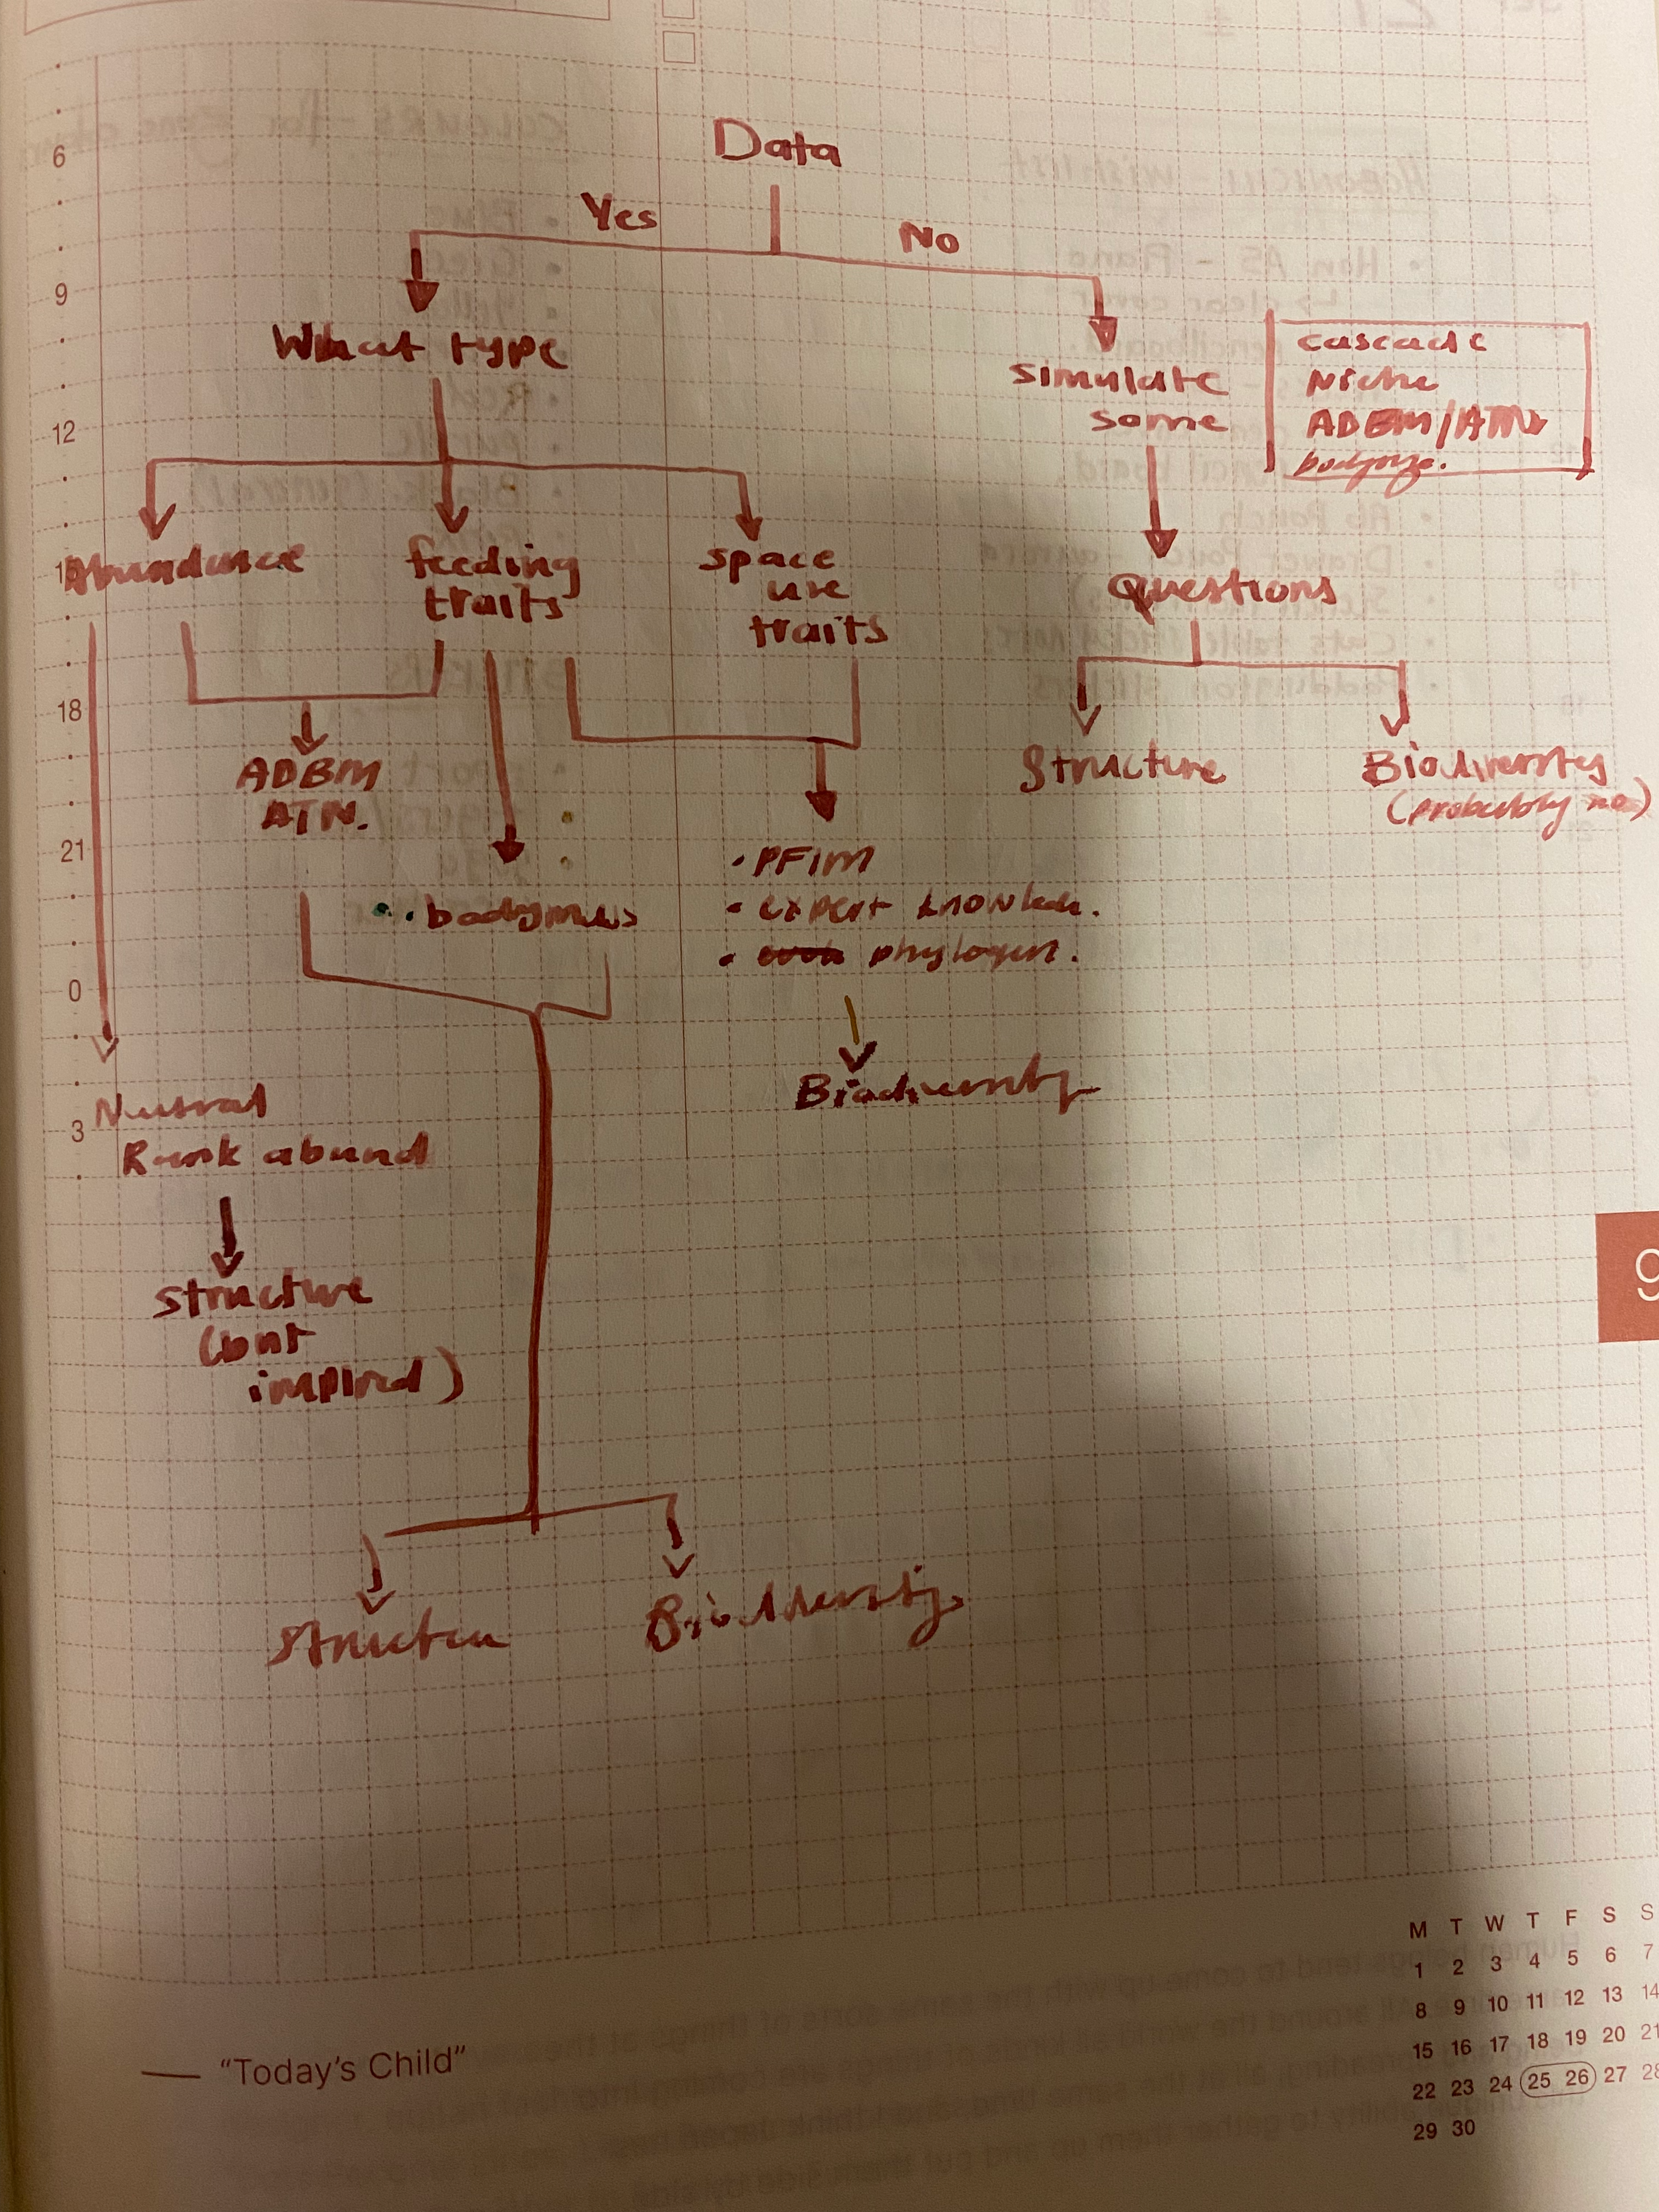
\includegraphics[keepaspectratio]{figures/guidelines.png}}

}

\caption{\label{fig-guidelines}TODO.}

\end{figure}%

\section*{References}\label{references}
\addcontentsline{toc}{section}{References}

\phantomsection\label{refs}
\begin{CSLReferences}{1}{0}
\bibitem[\citeproctext]{ref-allesina2008}
Allesina, S., Alonso, D., \& Pascual, M. (2008). A general model for
food web structure. \emph{Science}, \emph{320}(5876), 658--661.
\url{https://doi.org/10.1126/science.1156269}

\bibitem[\citeproctext]{ref-bambach2007}
Bambach, R. K., Bush, A. M., \& Erwin, D. H. (2007). Autecology and the
Filling of Ecospace: Key Metazoan Radiations. \emph{Palaeontology},
\emph{50}(1), 1--22.
\url{https://doi.org/10.1111/j.1475-4983.2006.00611.x}

\bibitem[\citeproctext]{ref-curtsdotter2011}
Curtsdotter, A., Binzer, A., Brose, U., De Castro, F., Ebenman, B.,
Eklöf, A., Riede, J. O., Thierry, A., \& Rall, B. C. (2011). Robustness
to secondary extinctions: Comparing trait-based sequential deletions in
static and dynamic food webs. \emph{Basic and Applied Ecology},
\emph{12}(7), 571--580. \url{https://doi.org/10.1016/j.baae.2011.09.008}

\bibitem[\citeproctext]{ref-delmas2018}
Delmas, E., Besson, M., Brice, M.-H., Burkle, L. A., Dalla Riva, G. V.,
Fortin, M.-J., Gravel, D., Guimarães, P. R., Hembry, D. H., Newman, E.
A., Olesen, J. M., Pires, M. M., Yeakel, J. D., \& Poisot, T. (2018).
Analysing ecological networks of species interactions. \emph{Biological
Reviews}, 112540. \url{https://doi.org/10.1111/brv.12433}

\bibitem[\citeproctext]{ref-dillon2022}
Dillon, E. M., Pier, J. Q., Smith, J. A., Raja, N. B., Dimitrijević, D.,
Austin, E. L., Cybulski, J. D., De Entrambasaguas, J., Durham, S. R.,
Grether, C. M., Haldar, H. S., Kocáková, K., Lin, C.-H., Mazzini, I.,
Mychajliw, A. M., Ollendorf, A. L., Pimiento, C., Regalado Fernández, O.
R., Smith, I. E., \& Dietl, G. P. (2022). What is conservation
paleobiology? Tracking 20 years of research and development.
\emph{Frontiers in Ecology and Evolution}, \emph{10}.
\url{https://doi.org/10.3389/fevo.2022.1031483}

\bibitem[\citeproctext]{ref-dunhill2024}
Dunhill, A. M., Zarzyczny, K., Shaw, J. O., Atkinson, J. W., Little, C.
T. S., \& Beckerman, A. P. (2024). Extinction cascades, community
collapse, and recovery across a Mesozoic hyperthermal event.
\emph{Nature Communications}, \emph{15}(1), 8599.
\url{https://doi.org/10.1038/s41467-024-53000-2}

\bibitem[\citeproctext]{ref-dunne2014}
Dunne, J. A., Labandeira, C. C., \& Williams, R. J. (2014). Highly
resolved early eocene food webs show development of modern trophic
structure after the end-cretaceous extinction. \emph{Proceedings of the
Royal Society B: Biological Sciences}, \emph{281}(1782), 20133280.
\url{https://doi.org/10.1098/rspb.2013.3280}

\bibitem[\citeproctext]{ref-erdos1959}
Erdős, P., \& Rényi, A. (1959). On random graphs. i. \emph{Publicationes
Mathematicae Debrecen}, \emph{6}(3-4), 290--297.
\url{https://doi.org/10.5486/pmd.1959.6.3-4.12}

\bibitem[\citeproctext]{ref-fricke2022}
Fricke, E. C., Hsieh, C., Middleton, O., Gorczynski, D., Cappello, C.
D., Sanisidro, O., Rowan, J., Svenning, J.-C., \& Beaudrot, L. (2022).
Collapse of terrestrial mammal food webs since the Late Pleistocene.
\emph{Science}, \emph{377}(6609), 1008--1011.
\url{https://doi.org/10.1126/science.abn4012}

\bibitem[\citeproctext]{ref-gauzens2025}
Gauzens, B., Thouvenot, L., Srivastava, D. S., Kratina, P., Romero, G.
Q., Berti, E., O'Gorman, E. J., González, A. L., Dézerald, O.,
Eisenhauer, N., Pires, M., Ryser, R., Farjalla, V. F., Rogy, P., Brose,
U., Petermann, J. S., Geslin, B., \& Hines, J. (2025). Tailoring
interaction network types to answer different ecological questions.
\emph{Nature Reviews Biodiversity}, 1--10.
\url{https://doi.org/10.1038/s44358-025-00056-7}

\bibitem[\citeproctext]{ref-gupta2022}
Gupta, A., Furrer, R., \& Petchey, O. L. (2022). Simultaneously
estimating food web connectance and structure with uncertainty.
\emph{Ecology and Evolution}, \emph{12}(3), e8643.
\url{https://doi.org/10.1002/ece3.8643}

\bibitem[\citeproctext]{ref-hao2025}
Hao, X., Holyoak, M., Zhang, Z., \& Yan, C. (2025). Global Projection of
Terrestrial Vertebrate Food Webs Under Future Climate and Land-Use
Changes. \emph{Global Change Biology}, \emph{31}(2), e70061.
\url{https://doi.org/10.1111/gcb.70061}

\bibitem[\citeproctext]{ref-jonsson2015}
Jonsson, T., Berg, S., Pimenov, A., Palmer, C., \& Emmerson, M. (2015).
The reliability of R50 as a measure of vulnerability of food webs to
sequential species deletions. \emph{Oikos}, \emph{124}(4), 446--457.
\url{https://doi.org/10.1111/oik.01588}

\bibitem[\citeproctext]{ref-jordano2016}
Jordano, P. (2016). Chasing Ecological Interactions. \emph{PLOS
Biology}, \emph{14}(9), e1002559.
\url{https://doi.org/10.1371/journal.pbio.1002559}

\bibitem[\citeproctext]{ref-kiessling2019}
Kiessling, W., Raja, N. B., Roden, V. J., Turvey, S. T., \& Saupe, E. E.
(2019). Addressing priority questions of conservation science with
palaeontological data. \emph{Philosophical Transactions of the Royal
Society B: Biological Sciences}, \emph{374}(1788), 20190222.
\url{https://doi.org/10.1098/rstb.2019.0222}

\bibitem[\citeproctext]{ref-milo2002}
Milo, R., Shen-Orr, S., Itzkovitz, S., Kashtan, N., Chklovskii, D., \&
Alon, U. (2002). Network motifs: Simple building blocks of complex
networks. \emph{Science}, \emph{298}(5594), 824--827.
\url{https://doi.org/10.1126/science.298.5594.824}

\bibitem[\citeproctext]{ref-morales-castilla2015}
Morales-Castilla, I., Matias, M. G., Gravel, D., \& Araújo, M. B.
(2015). Inferring biotic interactions from proxies. \emph{Trends in
Ecology \& Evolution}, \emph{30}(6), 347--356.
\url{https://doi.org/10.1016/j.tree.2015.03.014}

\bibitem[\citeproctext]{ref-petchey2008}
Petchey, O. L., Beckerman, A. P., Riede, J. O., \& Warren, P. H. (2008).
Size, foraging, and food web structure. \emph{Proceedings of the
National Academy of Sciences}, \emph{105}(11), 4191--4196.
\url{https://doi.org/10.1073/pnas.0710672105}

\bibitem[\citeproctext]{ref-pichler2023}
Pichler, M., \& Hartig, F. (2023). Machine learning and deep
learning{\textemdash}A review for ecologists. \emph{Methods in Ecology
and Evolution}, \emph{14}(4), 994--1016.
\url{https://doi.org/10.1111/2041-210X.14061}

\bibitem[\citeproctext]{ref-poisot2012}
Poisot, T., Canard, E., Mouquet, N., \& Hochberg, M. E. (2012). A
comparative study of ecological specialization estimators. \emph{Methods
in Ecology and Evolution}, \emph{3}(3), 537--544.
\url{https://doi.org/10.1111/j.2041-210x.2011.00174.x}

\bibitem[\citeproctext]{ref-rohr2010}
Rohr, R., Scherer, H., Kehrli, P., Mazza, C., \& Bersier, L.-F. (2010).
Modeling food webs: Exploring unexplained structure using latent traits.
\emph{The American Naturalist}, \emph{176}(2), 170--177.
\url{https://doi.org/10.1086/653667}

\bibitem[\citeproctext]{ref-roopnarine2006}
Roopnarine, P. D. (2006). Extinction cascades and catastrophe in ancient
food webs. \emph{Paleobiology}, \emph{32}(1), 1--19.
\url{https://www.jstor.org/stable/4096814}

\bibitem[\citeproctext]{ref-roopnarine2017}
Roopnarine, P. D. (2017). \emph{Ecological Modelling of Paleocommunity
Food Webs} (pp. 201--226). University of Chicago Press.

\bibitem[\citeproctext]{ref-schneider2016}
Schneider, F. D., Brose, U., Rall, B. C., \& Guill, C. (2016). Animal
diversity and ecosystem functioning in dynamic food webs. \emph{Nature
Communications}, \emph{7}(1), 12718.
\url{https://doi.org/10.1038/ncomms12718}

\bibitem[\citeproctext]{ref-shaw2024}
Shaw, J. O., Dunhill, A. M., Beckerman, A. P., Dunne, J. A., \& Hull, P.
M. (2024). \emph{A framework for reconstructing ancient food webs using
functional trait data} (p. 2024.01.30.578036). bioRxiv.
\url{https://doi.org/10.1101/2024.01.30.578036}

\bibitem[\citeproctext]{ref-stouffer2007}
Stouffer, D. B., Camacho, J., Jiang, W., \& Nunes Amaral, L. A. (2007).
Evidence for the existence of a robust pattern of prey selection in food
webs. \emph{Proceedings of the Royal Society B: Biological Sciences},
\emph{274}(1621), 1931--1940.
\url{https://doi.org/10.1098/rspb.2007.0571}

\bibitem[\citeproctext]{ref-strydom2021}
Strydom, T., Catchen, M. D., Banville, F., Caron, D., Dansereau, G.,
Desjardins-Proulx, P., Forero-Muñoz, N. R., Higino, G., Mercier, B.,
Gonzalez, A., Gravel, D., Pollock, L., \& Poisot, T. (2021). A roadmap
towards predicting species interaction networks (across space and time).
\emph{Philosophical Transactions of the Royal Society B: Biological
Sciences}, \emph{376}(1837), 20210063.
\url{https://doi.org/10.1098/rstb.2021.0063}

\bibitem[\citeproctext]{ref-thuiller2024}
Thuiller, W., Calderón-Sanou, I., Chalmandrier, L., Gaüzère, P.,
O'Connor, L. M. J., Ohlmann, M., Poggiato, G., \& Münkemüller, T.
(2024). Navigating the integration of biotic interactions in
biogeography. \emph{Journal of Biogeography}, \emph{51}(4), 550--559.
\url{https://doi.org/10.1111/jbi.14734}

\bibitem[\citeproctext]{ref-williams2000}
Williams, R. J., \& Martinez, N. D. (2000). Simple rules yield complex
food webs. \emph{Nature}, \emph{404}(6774), 180--183.
\url{https://doi.org/10.1038/35004572}

\bibitem[\citeproctext]{ref-williams2004}
Williams, R. J., \& Martinez, N. D. (2004). Stabilization of chaotic and
non-permanent food-web dynamics. \emph{The European Physical Journal B -
Condensed Matter}, \emph{38}(2), 297--303.
\url{https://doi.org/10.1140/epjb/e2004-00122-1}

\bibitem[\citeproctext]{ref-williams2008}
Williams, R. J., \& Martinez, N. D. (2008). Success and its limits among
structural models of complex food webs. \emph{The Journal of Animal
Ecology}, \emph{77}(3), 512--519.
\url{https://doi.org/10.1111/j.1365-2656.2008.01362.x}

\bibitem[\citeproctext]{ref-yeakel2014}
Yeakel, J. D., Pires, M. M., Rudolf, L., Dominy, N. J., Koch, P. L.,
Guimarães, P. R., \& Gross, T. (2014). Collapse of an ecological network
in ancient egypt. \emph{PNAS}, \emph{111}(40), 14472--14477.
\url{https://doi.org/10.1073/pnas.1408471111}

\end{CSLReferences}





\end{document}
